%!TEX TS-program = xelatex
%!TEX encoding = UTF-8 Unicode
%!TEX root = 2020-GS-ARTICLE.tex
%----------------------------------------------------------------- LANGUAGES ---
\newcommand{\mylanguages}{italian,english} % in reverse order
%---------------------------------------------------------- TITLE & SUBTITLE ---
\newcommand{\mytitle}{Ambiophonic Reverberation}
\newcommand{\mysubtitle}{For a more accessible and less technical introduction
                         to this topic, \\ see Introduction to General Relativity}
%----------------------------------------------------------------- AUTHOR(s) ---
\newcommand{\authorone}{Paradisi Francesco}
\newcommand{\institutione}{Conservatorio S. Cecilia di Roma}
\newcommand{\emailone}{francesco.paradisi10 @ gmail.com}
%-------------------------------------------------------------------------------
\newcommand{\authortwo}{Giuseppe Silvi}
\newcommand{\institutiontwo}{Conservatorio Nicolini di Bari}
\newcommand{\emailtwo}{silvi.giuseppe @ docenticonsba.it} % duplicate these 3 lines if more
%-------------------------------------------------------------------------------
\newcommand{\authorthree}{Edoardo Staffa}
\newcommand{\institutionthree}{Conservatorio S. Cecilia di Roma}
\newcommand{\emailthree}{edoardo.staffa1 @ gmail.com} % duplicate these 3 lines if more
%-------------------------------------------------------------- STYLE GS2020 ---
%!TEX TS-program = xelatex
%!TEX encoding = UTF-8 Unicode
%!TEX root = 2020-GS-ARTICLE.tex
%-------------------------------- PACKAGES AND OTHER DOCUMENT CONFIGURATIONS ---
\documentclass[
	a4paper,
	twocolumn
]{article}
\usepackage[
	top=20mm,
	bottom=25mm,
	textwidth=17.2cm,
	columnsep=0.8cm
]{geometry}
\usepackage[T1]{fontenc}
\usepackage[\mylanguages]{babel}
\usepackage{graphicx}
\usepackage{dblfloatfix}
\usepackage{graphicx}
\usepackage{epstopdf}
\epstopdfsetup{update}
\usepackage[usenames]{color}
\usepackage{xcolor}
\usepackage{amssymb}
\usepackage{hyperref} % For hyperlinks in the PDF
\usepackage{Alegreya}
\linespread{1.05}
\usepackage{
	fontspec,
	xltxtra,
	xunicode
	}
\usepackage{
	xfrac,
	unicode-math
	}

\defaultfontfeatures{Mapping=tex-text}
\setmonofont[
	Scale=MatchLowercase
	]{Andale Mono}
\setmathfont[
	Scale=MatchLowercase,
	Scale=1
	]{Libertinus Math}

\usepackage{microtype}

\usepackage[
	hang,
	small,
	labelfont=bf,
	up,
	textfont=it,
	up
	]{caption}
\usepackage{paralist} % For compact item lists
\usepackage{etoolbox} % Some tools: used for quote environment
\AtBeginEnvironment{quote}{\small}
\usepackage{titling} % Customizing the title section
\usepackage{booktabs} % Horizontal rules in tables
\usepackage{enumitem} % Customized lists
\setlist[itemize]{noitemsep} % Make itemize lists more compact
\usepackage{abstract} % Allows abstract customization
\renewcommand{\abstractnamefont}{\normalfont\bfseries} % Set the "Abstract" text to bold
\renewcommand{\abstracttextfont}{\normalfont\small\itshape} % Set the abstract itself to small italic text
\usepackage{titlesec} % Allows customization of titles
\renewcommand\thesection{\Roman{section}} % Roman numerals for the sections
\renewcommand\thesubsection{\Roman{subsection}} % roman numerals for subsections
\titleformat{\section}[block]{\large\centering}{\thesection.}{1em}{} % Change the look of the section titles
\titleformat{\subsection}[block]{\large}{\thesubsection.}{1em}{} % Change the look of the section titles
%------------------------------------------------------------- TITLE SECTION ---
\setlength{\droptitle}{-4\baselineskip} % Move the title up
\pretitle{\begin{center}\huge\bfseries} % Article title formatting
\posttitle{\end{center}} % Article title closing formatting
\title{\mytitle \\ \large{\emph{\mysubtitle}}} % Article title
\author{%
\textsc{\authorone}\\%
\normalsize \institutione \\ %
\normalsize \emailone%
\and
\textsc{\authortwo} \\%
\normalsize \institutiontwo \\ %
\normalsize \emailtwo %
\and
\textsc{\authorthree} \\%
\normalsize \institutionthree \\ %
\normalsize \emailthree %
}
\date{} % Leave empty to omit a date

\usepackage{fancyhdr} % Headers and footers
\pagestyle{fancy} % All pages have headers and footers
\fancyhead{} % Blank out the default header
\fancyfoot{} % Blank out the default footer
\fancyhead[C]{\small Ambiophonic Reverberation • Research Notes} % Custom header text
\fancyfoot[RO,LE]{\small \today~ • w: \input{includes/words.txt} • c: \input{includes/char.txt} • p:~\thepage} % Custom footer text
%-------------------------------------------------------------------------------
%-------------------------------------------------------------------------------
%	LISTINGS
%-------------------------------------------------------------------------------
%-------------------------------------------------------------------------------
\usepackage{listings}
% lstlistings setup
\definecolor{gsbg}{rgb}{0.98,0.98,0.98}

\lstset{%
  aboveskip=10pt,
	belowskip=5pt,
  language=C++,
  numbers=none,%left,%none,
  tabsize=4,
  %frame=single,
  breaklines=true,
  numberstyle=\tiny\ttfamily,
  backgroundcolor=\color{gsbg},
  basicstyle=\footnotesize\ttfamily,
  %commentstyle=\slshape\color{mylstcmt}, %\itshape,
  %frameround=tttt,
  columns=flexible, %fixed,
  showstringspaces=false,
  emptylines=2,
  inputencoding=utf8,
  extendedchars=true,
  literate=	{á}{{\'a}}1
			{à}{{\`a}}1
			{ä}{{\"a}}1
			{â}{{\^a}}1
			{é}{{\'e}}1
			{è}{{\`e}}1
			{ë}{{\"e}}1
			{ê}{{\^e}}1
			{ï}{{\"i}}1
			{î}{{\^i}}1
			{ö}{{\"o}}1
			{ô}{{\^o}}1
			{è}{{\`e}}1
			{ù}{{\`u}}1
			{û}{{\^u}}1
			{ç}{{\c{c}}}1
			{Ç}{{\c{C}}}1,
  emph={component, declare, environment, import, library, process},
  emph={[2]ffunction, fconstant, fvariable},
  emph={[3]button, checkbox, vslider, hslider, nentry, vgroup, hgroup, tgroup, vbargraph, hbargraph, attach},
  %emphstyle=\color{yotxt}, %\underline, %\bfseries,
  %morecomment=[s][\color{mylstdoc}]{<mdoc>}{</mdoc>},
  rulecolor=\color{black}
}

\usepackage[framemethod=tikz]{mdframed} % Allows defining custom boxed/framed environments

%-------------------------------------------------------------------------------
%--------------------------------------------------- INFORMATION ENVIRONMENT ---
%-------------------------------------------------------------------------------

% Usage:
% \begin{info}[optional title, defaults to "Info:"]
% 	contents
% 	\end{info}

\mdfdefinestyle{info}{%
	topline=false, bottomline=false,
	leftline=false, rightline=false,
	nobreak,
	singleextra={%
		\fill[black](P-|O)circle[radius=0.4em];
		\node at(P-|O){\color{white}\scriptsize\bf i};
		\draw[very thick](P-|O)++(0,-0.8em)--(O);%--(O-|P);
	}
}

% Define a custom environment for information
\newenvironment{info}[1][Info:]{ % Set the default title to "Info:"
	\medskip
	\begin{mdframed}[style=info]
		\noindent{\textbf{#1}}
}{
	\end{mdframed}
}

%-------------------------------------------------------------------------------
%----------------------------------------------------- BIOGRAFIA ENVIRONMENT ---
%-------------------------------------------------------------------------------

% Usage:
% \begin{bio}[optional title, defaults to "Info:"]
% 	contents
% 	\end{bio}

\mdfdefinestyle{bio}{%
	topline=false, bottomline=false,
	leftline=false, rightline=false,
	nobreak,
	singleextra={%
		\fill[black](P-|O)circle[radius=0.4em];
		\node at(P-|O){\color{white}\scriptsize\bf b};
		\draw[very thick](P-|O)++(0,-0.8em)--(O);%--(O-|P);
	}
}

% Define a custom environment for information
\newenvironment{bio}[1][Biografia:]{ % Set the default title to "Info:"
	\medskip
	\begin{mdframed}[style=bio]
		\noindent{\textbf{#1}}
}{
	\end{mdframed}
}

%-------------------------------------------------------------------------------
%------------------------------------------------------- WARNING ENVIRONMENT ---
%-------------------------------------------------------------------------------

% Usage:
% \begin{warn}[optional title, defaults to "Warning:"]
%	Contents
% \end{warn}

\mdfdefinestyle{warning}{
	topline=false, bottomline=false,
	leftline=false, rightline=false,
	nobreak,
	singleextra={%
		\draw(P-|O)++(-0.5em,0)node(tmp1){};
		\draw(P-|O)++(0.5em,0)node(tmp2){};
		\fill[black,rotate around={45:(P-|O)}](tmp1)rectangle(tmp2);
		\node at(P-|O){\color{white}\scriptsize\bf !};
		\draw[very thick](P-|O)++(0,-1em)--(O);%--(O-|P);
	}
}

% Define a custom environment for warning text
\newenvironment{warn}[1][Warning:]{ % Set the default warning to "Warning:"
	\medskip
	\begin{mdframed}[style=warning]
		\noindent{\textbf{#1}}
}{
	\end{mdframed}
}

%-------------------------------------------------------------------- ABSTRACT -
\renewcommand{\maketitlehookd}{%
\begin{abstract}
\noindent\input{includes/abstract.txt}
\end{abstract}
}

%------------------------------------------------------------ BEGIN DOCUMENT ---
\begin{document}
\maketitle
\thispagestyle{empty}
%-------------------------------------------------------------------- ABSTRACT -
% The abstract is an external txt file inside the includes folder
%-------------------------------------------------------------------------------

\section*{TO DO LIST}

\begin{compactitem}
\item descrizione generica dell'algoritmo di schroeder
\item le potenzialità dell'algoritmo
\item implementazione algoritmo in faust
\item allestimento dell'ambiophonic reverberation in sala concerto
\item implementazione esplicativa per Live Electronics
\item approfondimento bibliografico
\item conclusioni
\item
\item
\end{compactitem}



\section*{SCHROEDER - NATURAL SOUNDING ARTIFICIAL REVERBERATION}

%-------------------------------------------------------------------------------
\subsection*{DELAY FEEDBACK IN LOOP}

descrizione

%------------------------------------------------------
%------------------------- larghezza massima del codice
\begin{lstlisting}
//-------------------------- DELAY FEEDBACK IN LOOP ---
//
dfl(t,g) = (+ : @(t))~*(g);
\end{lstlisting}

descrizione

\begin{lstlisting}
//------------------ DELAY FEEDBACK IN LOOP - FIXED ---
//
dflc(t,g) = (+ : @(t-1))~*(g) : mem;
\end{lstlisting}

descrizione

\begin{lstlisting}
//-------------------------- DFL - FIXED - VARIABLE ---
//
dflcc(t,g) = (+ :
              de.delay(ma.SR/2, int(t-1)))~*(g) : mem;
\end{lstlisting}

%-------------------------------------------------------------------------------
\subsection*{ALL-PASS FILTER}

%------------------------------------------------------
%------------------------- larghezza massima del codice
\begin{lstlisting}
//--------------------------------- ALL-PASS FILTER ---
//
apf(t,g) = _ <: *(-g)+(dflcc(t,g)*(1-(g*g)));
\end{lstlisting}

%-------------------------------------------------------------------------------
\subsection*{T60}
%------------------------------------------------------
%------------------------- larghezza massima del codice
\begin{lstlisting}
//--------------------------------------------- T60 ---
// For a feedback loop with open loop gain g, the sound
// level decay by -20*log(g) decibels for every trip
// around the feedback loop. Since every round trip
// takes t second, the time for a 60dB decay is
//
msT60(t,g) = (60/(-20*log10(g)))*t;
process = msT60(0.1,0.708); // 2 seconds
\end{lstlisting}

\subsection*{ALL-PASS REVERBERATOR}
%------------------------------------------------------
%------------------------- larghezza massima del codice
\begin{lstlisting}
//------------------------ INCREASE OF ECHO DENSITY ---
// The delay of each section is made about 1/3 of the
// preceding delay. Thus, the delay of the n-th unit
// will be t1(1/3)^n-1. The gains are most conveniently
// made equal to about 0.7. [...] The effective echo
// density of 5 loops in series will be approximately
// 81/t1. For t1 = 0.1 sec, the effective echo density
// will be 810 per second which is sufficiently close
// to the required 1000 per second. To avoid echo
// cancellation and superposition, it is advisable to
// use incommensurate delay ratios rather than the
// round number 3.
//
ied5 = apf(5507,0.7) :
       apf(1831,0.7) :
       apf(613,0.7) :
       apf(199,0.7) :
       apf(67,0.7);
\end{lstlisting}

\subsection*{NON-EXPONENTIAL DECAY}
%------------------------------------------------------
%------------------------- larghezza massima del codice
\begin{lstlisting}
//--------- MIXING OF DIRECTSOUND AND REVERBERATION ---
//--------------------------- NON-EXPONENTIAL DECAY ---
//
dflr(t,g) = (+ : de.delay(ma.SR/2, int(t-1)) :
             ied5)~*(g) : mem;
aprdw(t,g) = _ <: *(-g)+(dflr(t,g)*(1-(g*g)));
\end{lstlisting}

\subsection*{COMB FILTER REVERBERATION}
%------------------------------------------------------
%------------------------- larghezza massima del codice
\begin{lstlisting}
//------------------------ THE COMB FILTER APPROACH ---
// The values of the delays t1 through t4 are spread
// [...] between 30 and 45 ms here in prime numbers at
// 48KHz from 1440 to 2160 samples.
//
schrev = _ <: // to 4 parallel comb
  dflc(1447,0.812),
  dflc(1721,0.78),
  dflc(1873,0.76),
  dflc(2161,0.74) :>
  apf(83,0.7) : apf(229,0.7);
//
// components in reverse order
// two allpass to 4 comb
//
revsch = apf(83,0.7) : apf(229,0.7) <:
  dflc(1447,0.812),
  dflc(1721,0.78),
  dflc(1873,0.76),
  dflc(2161,0.74);
// commutability test
//
process = os.impulse <: schrev, (revsch :> _);
\end{lstlisting}

\subsection*{FREQUENCY-DEPENDENT REVERBERATION TIME}
%------------------------------------------------------
%------------------------- larghezza massima del codice
\begin{lstlisting}
//----------------- FREQUENCY-DEPENDENT REVERB TIME ---
// If it is desired to make the reverberation time a
// function of frequency, the gains g1 through g4 in
// have to be made frequency dependent. For this, a
// simple RC-section in each feedback loop will
// suffice. In this manner further realism can be added
// to the artificial reverberation by making the
// reverberation time larger for the low frequencies.
// This trend of reverberation time with frequency is
// typical of many concert halls and cathedrals.
//
dflf(t,g,fc) = (+ : de.delay(ma.SR/2,
             int(t-1)))~scy.onepole(fc)*(g) :
             mem;
//
schfdrevt = _ <: // to 4 parallel comb
  dflf(1447,0.812,5000),
  dflf(1721,0.78,4000),
  dflf(1873,0.76,3000),
  dflf(2161,0.74,2000) :>
  apf(83,0.7) : apf(229,0.7);
\end{lstlisting}

Descrizione

%------------------------------------------------------
%------------------------- larghezza massima del codice
\begin{lstlisting}
//-------------------------------- max-msp onepole~ ---
onepole(fc) = *(a) : +~*(ac)
with{
    a= sin(abs(fc)*2*ma.PI/ma.SR) : clip(0,1);
    ac = 1-a;
};
\end{lstlisting}

\section*{NEXT PRIME}
%------------------------------------------------------
%------------------------- larghezza massima del codice
\begin{lstlisting}
#include <stdio.h>
#include <math.h>

int is_prime(int num);
int next_pr(int num);

int next_pr(int num){
  int c;
  if(num < 2)
    c = 2;
  else if (num == 2)
    c = 3;
  else if(num & 1){
    num += 2;
    c = is_prime(num) ? num : next_pr(num);
  } else
    c = next_pr(num-1);

    return c;
}

int is_prime(int num){
  if((num & 1)==0)
    return num == 2;
  else {
    int i, limit = sqrt(num);
    for (i = 3; i <= limit; i+=2){
    if (num % i == 0)
    return 0;
    }
  }
  return 1;
}
\end{lstlisting}

%------------------------------------------------------
%------------------------- larghezza massima del codice
\begin{lstlisting}
np = ffunction(int next_pr(int), <nextprime.h>,"");
\end{lstlisting}

\section*{AMBIOPHONIC REVERBERATION}

\begin{quote}
  This procedure, which is already obsolete, makes use of delaying devices
  reproducing not only the discrete initial reflections; but also the
  reverberation tail. The reflection sequences have herewith to be chosen in
  such a way that no comb-filter effects, such as flutter echoes, will be
  produced with impulsive music motifs. The functioning of a simple ambiophonic
  system can be described as follows: to the direct sound emanating directly
  from the original source and directly irradiated into the room, there are
  admixed delayed signals produced by an adequate sound delaying system (in the
  initial stages this was just a magnetic sound recording system) which are
  then irradiated like reflections arriving with corresponding delay from the
  walls or the ceiling. This requires additional loudspeakers appropriately
  distributed in the room for irradiating the delayed sound as diffusely as
  possible. For further delaying the sound it is possible to arrange an additional
  feedback from the last output of the delay chain to the input. A system of this
  kind was first suggested by Kleis51 and was installed realized in several large
  halls. 52, 53 \cite{gb:08}
  % [51]. D. Kleis, “Moderne Beschallungstechnik” (Modern Sound Reinforcement). Philips tech. Rdsch. 20 (1958/59) 9, S. 272ff. und 21 (1959/60) 3, S. 78ff.
  % [52]. E. Meyer, and H. Kuttruff, “Zur Raumakustik einer großen Festhalle” (Regarding the Room Acoustic of a Large Festival Hall), Acustica 14 (1964) 3, S. 138–147.
  % [53]. W. Kaczorowski, “Urzadzenia elektroakustyczne i naglosnia w Wojewodzkiej Hali Widowiskowo-Sportowej w Katowicach” (Electroacoustic Equipment in the Wojewod Sport Hall in Katowice). Technika Radia i Telewizji 4 (1973) S. 1–16.
\end{quote}

\begin{quote}

In 1965, the thirty-four-year-old studio
received a much-deserved facelift, including the installment of a state-of-the-
art ambiophonics system. The brainchild of Gilbert Dutton, the head of EMI’s
research labs, the ambiophonics system was designed to increase Studio 1’s
short reverb time, which typically clocked in around two seconds. The idea
behind Dutton’s innovation was to afford the spacious studio with the sound and feel of a concert hall.
The ambiophonic process, as Dutton devised it, was relatively simple. The microphones in the studio sent a slightly delayed signal that would be played back through a series of loudspeakers installed on the walls of the mammoth room. The new signal would be picked up, in turn, by the original set of microphones and recorded. In Dutton’s design, an increase in reverb would be realized by virtue of the length of the delay and the distance between the speakers and the mics. Dutton’s ambiophonic system required ninety-six loudspeakers in order to create the necessary sound diffusion. Historian Howard Massey has described ambiophonics as “the Grand Experiment that never quite worked.” And in truth, the whole apparatus fell somewhat short of Dutton’s original ambition for creating a kind of midcentury forerunner of contemporary surround sound.
Given the limitations of 1960s-era technology, the system maxed out after six signal delays—a
process that was made possible by the installation of a “delay drum,” which
consisted of a rotating metal platter, its outer edge having been treated with
ferric oxide, with seven magnetic heads (one for recording, six for playback)
randomly interspersed around its perimeter. Each of the playback heads
directed its signal to a preamplifier, which returned the signal to sixteen of the
loudspeakers installed on the walls of Studio 1. As Massey explained, “The
whole system was essentially a large feedback loop, and therein lay the rub: It
only functioned best when on the verge of howling, which made it largely
uncontrollable.” For his part, Townsend concurred, feeling that ambiophonics
“was too artificial. The results sounded a little phony.” In many ways,
Dutton’s system was just another one of the several discrete elements that
needed to come together on that magical evening to bring George and the Beatles' vision for "A Day in The Life" into reality.

\end{quote}


\section*{ALGORITMO}

\begin{lstlisting}
import("stdfaust.lib");
// ------ comb
//
dflc(t, g) = (+ : de.delay(ma.SR, int(t-1)))~*(max(0, min(0.999, g))) : mem;
// ------ allpass
//
alp(t, g) = _<:(_*(ma.neg(max(0.5, min(0.9, g)))))+(dflc(t, g)*(1-(g*g)));
// ------ filtro passa basso "onepole" Dattorro inspired
//
lp1p(a) = *(a) : + ~ *(1-a);
// ------ sliders feedback
//
g(x) = hgroup("[01]CONTROL",x);
  gr(x) = g(hgroup("feedback", x));
      fbkc = gr(hslider("[02]DIFFUSION [style:knob]", 0.708, 0, 0.9, 0.01));
      fbk = gr(hslider("[03]FB FDN [style:knob]", 0.708, 0, 0.99, 0.01) : si.smoo) ;
      fbka = gr(hslider("[01]INPUT AP [style:knob]", 0.708, 0, 0.99, 0.01) : si.smoo);
      fbkm = gr(hslider("[04]MATRIX [style:knob]", 0.708, 0, 0.99, 0.01) : si.smoo);
// ------ slider filtro
//
glp(x)  = g(hgroup("filtro",x));
  bandwidth = glp(hslider("BANDWIDTH [style:knob]", 0.9995, 0.0001, 0.9999999, 0.0000001));
  damping = glp(hslider("DAMPING [style:knob]", 0.1, 0, 0.999, 0.001));
// ------ sliders x lunghezza, y altezza, z profondità, le variabili con p indicano la sorgente rispetto alla stanza
//
xg(x) = hgroup("[02]ROOM", x);
  yg(x) = xg(hgroup("vertical", x));
      size = xg((hslider("SIZE [style:knob]",1,0,2,0.01)));
      x = ((size*(7)));
      y = ((size*(5)));
      z = ((size*(3)));
      xps = xg(hslider("Position",0.5,0,1,0.01));
// ------ position values limitati ai valori x,y,z
//
xp = x*xps : np;
// ------ 2 allpass in serie + offset L/R
//
/*ambs(i) =  ambiserie*i, ambiserie*(1-i)
  with{
      ambiserie = alp(142, fbka) : alp(307, fbka) : alp(107,fbka) : alp(277, fbka) : alp(311, fbka) : alp(59, fbka);
  };*/
//ambiserie = alp(142, fbka) : alp(307, fbka) : alp(107,fbka) : alp(277, fbka) : alp(311, fbka) : alp(59, fbka);
primeseq(n) = seq(i,n,np);
ambis(fedb, n) = seq(i, n, alp(pm.l2s(2:primeseq(i+1)),fedb));
// ------ route + feedback delay network, 6 comb controllati dagli slider
//
ambifdn4(pippo,n) = (xroute :((alpar(x-xp,fbkc,pippo))*(xps)), ((alpar(xp,fbkc,pippo))*(1-xps)), (alpar(y,fbkc,pippo)) , (alpar(z,fbkc,pippo))) ~ (xfbk(n) : feedbackmatrix(n)) : rut
  with {
      xroute(a,b,c,d,a1,b1,c1,d1)=a+a1,b+b1,c+c1,d+d1; // route del segnale in ingresso per le somme
      feedbackmatrix(N) = bhadamard(N);
      vbutterfly(n) = si.bus(n) <: (si.bus(n):>bus(n/2)) , ((si.bus(n/2),(si.bus(n/2):par(i,n/2,*(-1)))) :> si.bus(n/2));
      bhadamard(2) = si.bus(2) <: +,-;
      bhadamard(n) = si.bus(n) <: (si.bus(n):>si.bus(n/2)) , ((si.bus(n/2),(si.bus(n/2):par(i,n/2,*(-1)))) :> si.bus(n/2))
               : (bhadamard(n/2) , bhadamard(n/2));
      xfbk(n) = par(i,n,lp1p(damping)*(fbk)*(1/sqrt(n)));
      alpar(sb, fb, N)=seq(i,N,alp(pm.l2s(sb:primeseq(i+1)),fb));
      rut(l, r ,y, z)=l+((y+z)*0.5),r+((y+z)*0.5);
      //xfbk1 = par(i) // feedback
  };
// ------ Reverb systems
//
ambidat2ch(pipp) = lp1p(bandwidth) // <: ambis(fbka, n)
                                   <: ambifdn4(pipp,4); // --- 2 canali ---
ambidat6ch = lp1p(bandwidth) <: ambs(xps) <: ambifdn6 : sixroute // --- 6 canali ---
  with{
      sixroute(a,b,c,d,e,f) = a,c,e,b,d,f; // route per il segnale L/R nel caso dei 6 canali
  };
// ------ process
//
process = ambidat2ch(4);
//process = alpar(primes,fbkc,16);
alpar(t, fb, N) = seq(i,N,alp((t/((i+1)/2)):np,fb));//ambidat2ch(4);
primes = xg((hslider("PRIMES [style:knob]",2,2,24000,1)));
np = ffunction(int next_pr(int), <nextprime.h>,"");

dist = vslider("distance", 1,0.01,20,0.01);

//process = deltime(pm.l2s(dist)) : vbargraph("primo",2,pow(2,30));
\end{lstlisting}

% \begin{warn}[Einstein's theory]
% has important astrophysical implications. For example, it
% implies the existence of black holes regions of space in which space and time
% are distorted in such a way that nothing, not even light, can escape as an
% end state for massive stars.
% \end{warn}
%
%
% %-------------------------------------------------------------------------------
% \subsubsection*{UNNUMBERED SUB-SUB-SECTION}
% Some predictions of general relativity differ significantly from those of
% classical physics, especially concerning the passage of time, the geometry of
% space, the motion of bodies in free fall, and the propagation of light. Examples
% of such differences include gravitational time dilation, gravitational lensing,
% the gravitational redshift of light, and the gravitational time delay. The
% predictions of general relativity in relation to classical physics have been
% confirmed in all observations and experiments to date. Although general
% relativity is not the only relativistic theory of gravity, it is the simplest
% theory that is consistent with experimental data. However, unanswered questions
% remain, the most fundamental being how general relativity can be reconciled with
% the laws of quantum physics to produce a complete and self-consistent theory of
% quantum gravity.
%
% Einstein's theory has important astrophysical implications. For example, it
% implies the existence of black holes regions of space in which space and time
% are distorted in such a way that nothing, not even light, can escape as an
% end state for massive stars. There is ample evidence that the intense radiation
% emitted by certain kinds of astronomical objects is due to black holes. For
% example, microquasars and active galactic nuclei result from the presence of
% stellar black holes and supermassive black holes\ldots
%
%
% \vfill\null
%
% \begin{figure}[b]
% \begin{center}
% 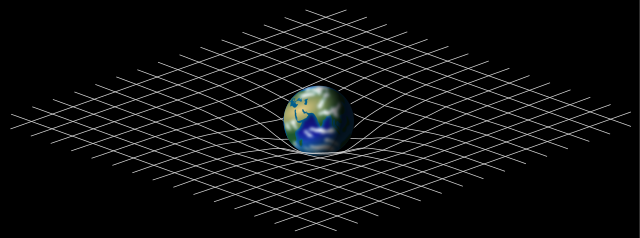
\includegraphics[width=.47\textwidth]{img/image1.png}
% \caption{\textbf{Spacetime curvature schematic}. Lattice analogy of the deformation
% of spacetime caused by a planetary mass.}
% \label{gr01}
% \end{center}
% \end{figure}
%
% \newpage % USE NEWPAGE TO FORCE COLUMNN INTERRUPTION
% %-------------------------------------------------------------------------------
% %-------------------------------------------------------------------------------
% \section*{UNNUMBERED SECTION}
%
% \begin{quote}
% La musica non e` solo composizione. \\
% Non è artigianato, non è un mestiere. \\
% La musica è pensiero. \cite{nono85}
% \end{quote}
%
% Some predictions of general relativity differ significantly from those of
% classical physics, especially concerning the passage of time, the geometry of
% space, the motion of bodies in free fall, and the propagation of light. Examples
% of such differences include gravitational time dilation, gravitational lensing,
% the gravitational redshift of light, and the gravitational time delay. The
% predictions of general relativity in relation to classical physics have been
% confirmed in all observations and experiments to date. Although general
% relativity is not the only relativistic theory of gravity, it is the simplest
% theory that is consistent with experimental data. However, unanswered questions
% remain, the most fundamental being how general relativity can be reconciled with
% the laws of quantum physics to produce a complete and self-consistent theory of
% quantum gravity.
%
% \begin{table}[htp]
% \begin{center}
% \begin{tabular}{ll}
% \textbf{Stages} & \textbf{Dur.} \\
% \hline
% \textbf{Omnidirectional Expositions} & 6 mo. \\
% Sound-shape analysis and visualizations & \\
% Sound-shape reproduction & \\
% Sound-shape database design & \\
% \hline
% \textbf{Micro-Rhythm of sound-shape} & 12 mo. \\
% Solo repertoire analysis & \\
% Sound-shape explosion in practising & \\
% From literature to shapes open-data & \\
% \hline
% \textbf{Rhythm of sound-shape interactions} & 12 mo. \\
% Multiple sources multiple shapes & \\
% Relationship and complexity perception & \\
% \hline
% \textbf{Sound-shape in musical composition} & 12 mo. \\
% AI: unleashed writing opportunities & \\
% AI: can you listen the time? & \\
% \hline
% \textbf{Final documentation} & 6 mo. \\
% \end{tabular}
% \label{timesheet}
% \caption{Thinking Tetrahedral Today stages}
% \end{center}
% \end{table}%
%
% Einstein's theory has important astrophysical implications. For example, it
% implies the existence of black holes regions of space in which space and time
% are distorted in such a way that nothing, not even light, can escape as an
% end state for massive stars. There is ample evidence that the intense radiation
% emitted by certain kinds of astronomical objects is due to black holes. For
% example, microquasars and active galactic nuclei result from the presence of
% stellar black holes and supermassive black holes, respectively. The bending of
% light by gravity can lead to the phenomenon of gravitational lensing, in which
% multiple images of the same distant astronomical object are visible in the sky.
% General relativity also predicts the existence of gravitational waves, which
% have since been observed directly by the physics collaboration LIGO. In addition,
% general relativity is the basis of current cosmological models of a consistently
% expanding universe. \cite{gerzon_70b}
%
% \begin{compactitem}
% \item Derivations of the Lorentz transformations
% \item Einstein–Hilbert action
% \item Tests of general relativity
% \item Two-body problem in general relativity
% \end{compactitem}
%
% \begin{figure}[t]
% \centering
% 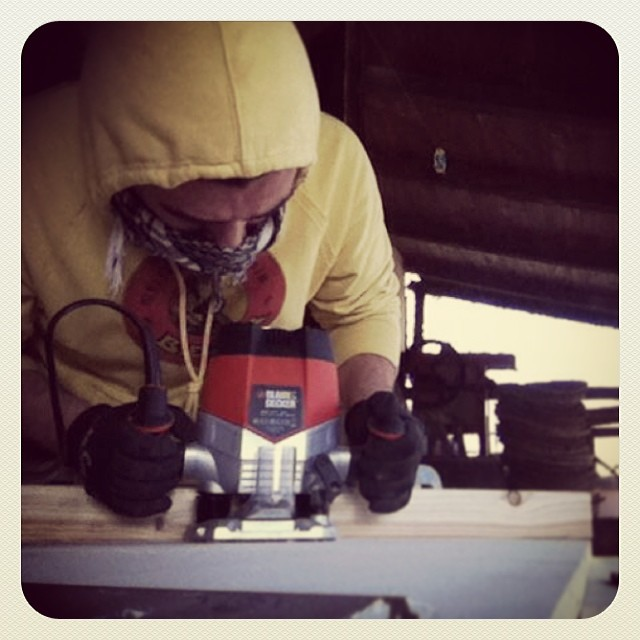
\includegraphics[width=.47\textwidth]{img/image2.jpg}
% \caption{Mind Mapping}
% \label{gs}
% \end{figure}
%
% \begin{equation}
% m(x,p,\theta) = (p*x) + ((1-p)*(x\cos\theta)
% \label{eq:mid}
% \end{equation}
%
% Some predictions of general relativity differ significantly from those of
% classical physics, especially concerning the passage of time, the geometry of
% space, the motion of bodies in free fall, and the propagation of light.
%
% %--------------------------------------------
% %----------------larghezza massima del codice
% \begin{lstlisting}
% dflc(t, g) = (+ : de.delay(ma.SR, int(t-1)))~*(max(0, min(0.999, g))) : mem;
% \end{lstlisting}
%
% Examples of such differences include gravitational time dilation, gravitational
% lensing, the gravitational redshift of light, and the gravitational time delay.
% The predictions of general relativity in relation to classical physics have been
% confirmed in all observations and experiments to date.

\vfill\null

\raggedright
\bibliographystyle{unsrt}
\bibliography{includes/bibliography.bib}

\end{document}

%%%%%%%%%%%%%%%%%%%%%%%%%%%%%%%%%%%%%%%%%%%%%%%%%%%%%%%%%%%%%%%%%%%%%%%%%%%%%%%%
% 2020 GIUSEPPE SILVI ARTICLE TEMPLATE BASED ON
%%%%%%%%%%%%%%%%%%%%%%%%%%%%%%%%%%%%%%%%%%%%%%%%%%%%%%%%%%%%%%%%%%%%%%%%%%%%%%%%
% Journal Article
% LaTeX Template
% Version 1.4 (15/5/16)
% This template has been downloaded from:
% http://www.LaTeXTemplates.com
% Original author:
% Frits Wenneker (http://www.howtotex.com) with extensive modifications by
% Vel (vel@LaTeXTemplates.com)
% License:
% CC BY-NC-SA 3.0 (http://creativecommons.org/licenses/by-nc-sa/3.0/)
%%%%%%%%%%%%%%%%%%%%%%%%%%%%%%%%%%%%%%%%%%%%%%%%%%%%%%%%%%%%%%%%%%%%%%%%%%%%%%%%
